La gestion d'équipe, ça n'est pas un tâche facile. La gestion du projet en parallèle, encore moins. Et le déploiement de l'ensemble des systèmes mis en place par l'équipe, plus qu'un challenge.

\section{Agile \& SCRUM}

La méthodologie de travail que nous avons choisi d'adopter s'inspire de la méthodologie Agile et des principes SCRUM. L'Agile a clairement ses avantages par rapport à d'autres méthodologies de travail. Cependant, les restrictions suivantes a rendu notre méthodologie moins "agile" que l'on aurait espérer:

\begin{itemize}
    \item La contrainte du temps: le projet devait être développer sous 3-4 mois. La méthodologie Agile permet le suivi d'un projet plus efficace et avec un rendement amélioré, au détriment du temps, cependant. Cela veut dire que nous prenons plus de temps à mettre en place le projet pour que ce dernier soit qualitatif et que le suivi de ce dernier soit aisé. Malheureusement, le principe de manque de temps sera le leitmotiv récurrent de ce rapport.
    \item La contrainte de l'école: un peu liée avec la contrainte précédente, le fait que l'on soit à l'école restreint certaines choses. Premièrement, nous devons travailler pour d'autre cours en parallèle, ce qui ralenti encore plus le développement. Ensuite, un des principes agiles est de faire une réunion quotidienne (et matinale) d'une dizaine de minutes afin de receuillir l'avancement de chacun. A la place d'une réunion quotidienne, nous avons opté pour une réunion hebdomadaire, mais cela ne valait pas une réunion quotidienne.
\end{itemize}

Ce genre de méthodologie requiert aussi une grande analyse du projet à l'avance, ce qui a été compliqué au départ. J'ai moi-même voulu commencer à travailler ce projet assez tôt, mais l'énoncé de ce dernier nous a été parvenu qu'un mois après mon pic de motivation. De plus, l'énoncé a été une part de difficulté dans notre façon de faire car nous avions dû déchiffrer certaines parties, et cela nous a pris pas mal de temps.

\section{YouTrack: notre outil de gestion de projet}

Afin de gérer les différentes deadlines et les tâches assignées à certains projets, j'ai décidé de partir sur un hébergement sur le cloud d'une version gratuite de YouTrack.

\begin{figure}[H]
    \centering
    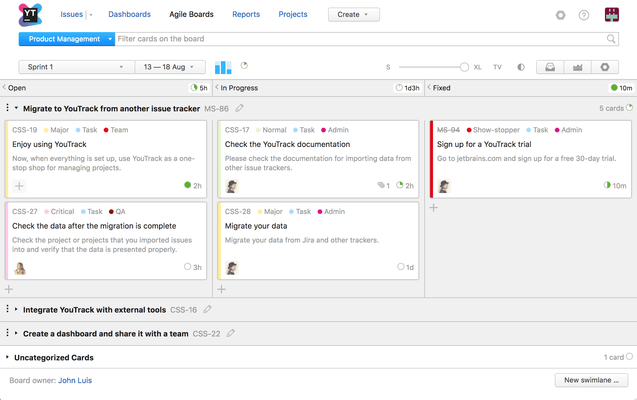
\includegraphics[width=\textwidth]{./img/youtrack.png}
    \caption{Exemple de l'interface de YouTrack (non représentatif de notre projet)}
    \label{fig:youtrack}
\end{figure}

La customisation et la classification des différentes tâches est totalement customisable par l'administrateur de YouTrack (c'est-à-dire moi). Ensuite, les utilisateurs vont pouvoir créer leur tâches en leur assignant un projet, l'importance de la tâche, le temps passé dessus, le temps estimé\dots enfin bref, quelques paramètres bien sympatique au suivi du projet. De plus, il y avait moyen d'afficher un Gantt Chart, ce qui permettait de voir l'avancée du projet et les différentes deadlines des tâches.

\begin{figure}[H]
    \centering
    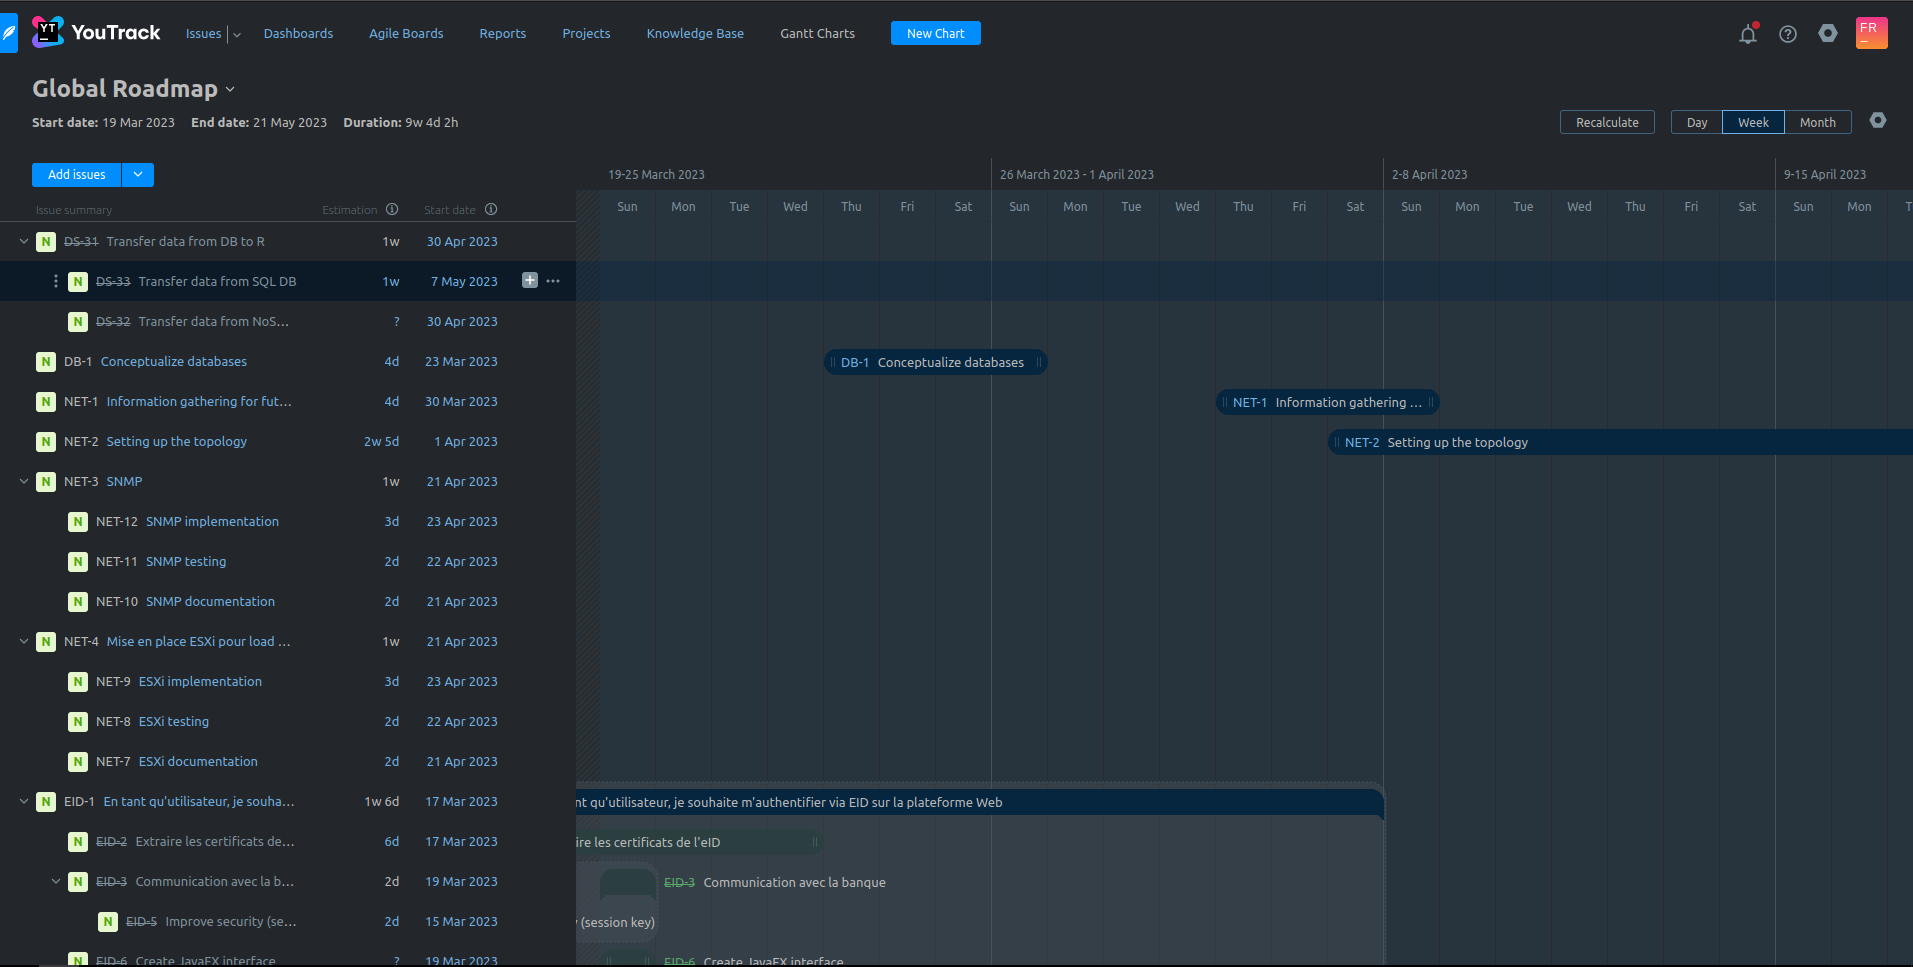
\includegraphics[width=\textwidth]{./img/youtrack-gantt.png}
    \caption{Vue du projet sous un graphe de Gantt}
    \label{fig:youtrack-gantt}
\end{figure}

\section{Difficultées encourrues}

\subsection{L'organisation des rôles}

L'une des premières difficulté qu'on a rencontré en tant qu'équipe est la réassignation des rôles. Étant une équipe avec moins de pairs qu'estimé initialement (8 à la place de 9), certains rôles n'étaient pas assignables. Joignez à ça la vague idée que l'on avait du projet au début, et ça nous compliquait l'assignation des rôles. Finalement, nous nous étions mis d'accord sur un tableau de rôles.

\begin{figure}[H]
    \centering
    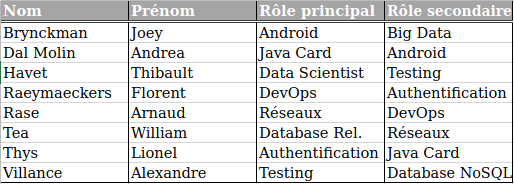
\includegraphics[width=\textwidth]{./img/roles.png}
    \caption{Tableau des rôles rendu au professeur responsable}
    \label{fig:roles}
\end{figure}

En tant qu'étudiante bachelière ayant suivi une formation de développement d'applications, ce principe de rôle m'eût parut bizarre. De fait, si cette contrainte n'était pas à rendre si tôt ni même existante, je pense que j'aurais: soit annuler toute notion de "rôle", et de naturellement laisser les personnes se diriger vers ce qui leur plaît (certains aurait peut-être préféré développer que de faire du réseau, par exemple), soit assigner les rôles après avoir analyser les différentes parties du projet (même si je préfère clairement la première approche). L'avantage aussi de cette première approche est que, si quelqu'un bloque sur une tâche, un autre pourra se permettre de l'aider ou bien de reprendre sa tâche et de tout de même avancer, surtout si c'est une tâche critique.

Un autre gros soucis avec la méthodologie des rôles, est que, vers la fin du projet, nous nous sommes retrouvé avec certains qui avait moins contribué que d'autres car leur rôle n'avait aucun sens comparé aux autres. La charge des différents rôles était déjà difficilement estimable, mais en plus nous nous sommes rendus compte de l'inégalité de ladite charge.

\subsection{Préparation \& Analyse du projet}

L'analyse de l'énoncé du projet était une étape fastidieuse. Premièrement, on ne savait pas réellement où donner de la tête. Là où certains avait beaucoup à analyser à cause de leur rôle (i.e. Joey et la conception de l'applcation mobile), d'autre n'avaient pas réellement beaucoup à faire car une analyse n'était pas vraiment nécessaire (i.e. les bases de données relationnelles). Cette étape était très importante car il eut fallu, au final, transformer cet énoncé en User Stories à encoder dans l'outil de gestion de projet. Malheureusement, même si nous avons eu en globalité quelques User Stories intéressantes, l'utilisation de ces dernières n'a pas été au plus efficace.

\subsection{Le testing}

Si vous avez l'oeil, vous aurez remarqué que nous ne parlons pas énormément du testing. Autant certain l'ont appliqué localement, c'est-à-dire qu'ils ont mis en place des tests unitaires. Autant, globalement, ça n'était pas supervisé ni même encouragé. Et, ça été plus un manque de gestion général que le problème de la personne responsable du testing. Le but était le suivant: Analyser l'application, mettre en place des User Stories, faire des tests basés sur ces User Stories et puis enfin implémenter la solution. Cependant, c'est premièrement quelque chose qui, comme pour la méthodologie agile, demande plus de temps qu'initalement car nous avons besoin de mettre en place tout les tests derrière avant le commencement du développement. Encore une fois quelque chose qui demande du temps.

Je suis une des premières à dire que le testing est une étape très importante dans le développement et la mise en place d'une solution logicielle. Cependant, qu'aurions nous fait si, à la finalité du projet, nous aurions tous les tests soigneusement écrits, mais aucune implémentation concrète de la solution de l'énoncé ?

